\documentclass[a4paper,10pt, notitlepage]{report}
\usepackage[utf8]{inputenc}
\usepackage{natbib}
\usepackage{amssymb}
\usepackage{amsmath}
\usepackage{enumitem}
\usepackage{xcolor}
\usepackage{cancel}
\usepackage{mathtools}
\usepackage[portuguese]{babel}

%%%%%%%%%%%%%%%%%%%% Notation stuff
\newcommand{\pr}{\operatorname{Pr}} %% probability
\newcommand{\vr}{\operatorname{Var}} %% variance
\newcommand{\rs}{X_1, X_2, \ldots, X_n} %%  random sample
\newcommand{\irs}{X_1, X_2, \ldots} %% infinite random sample
\newcommand{\rsd}{x_1, x_2, \ldots, x_n} %%  random sample, realised
\newcommand{\bX}{\boldsymbol{X}} %%  random sample, contracted form (bold)
\newcommand{\bx}{\boldsymbol{x}} %%  random sample, realised, contracted form (bold)
\newcommand{\bT}{\boldsymbol{T}} %%  Statistic, vector form (bold)
\newcommand{\bt}{\boldsymbol{t}} %%  Statistic, realised, vector form (bold)
\newcommand{\emv}{\hat{\theta}}
\DeclarePairedDelimiter\ceil{\lceil}{\rceil}
\DeclarePairedDelimiter\floor{\lfloor}{\rfloor}

% Title Page
\title{Segunda avaliação (A2)}
\author{Disciplina: Inferência Estatística \\ Instrutor: Professor Carvalho}
\date{03 de Dezembro de 2020}

\begin{document}
\maketitle

% \textbf{Data de Entrega: 19 de Agosto de 2020.}

\begin{center}
\fbox{\fbox{\parbox{1.0\textwidth}{\textsf{
    \begin{itemize}
        \item Por favor, entregue um único arquivo PDF;
        \item O tempo para realização da prova é de 3 horas, mais vinte minutos para upload do documento para o e-class;
        \item Leia a prova toda com calma antes de começar a responder;
        \item Responda todas as questões sucintamente;
        \item Marque a resposta final claramente com um quadrado, círculo ou figura geométrica de sua preferência;
        \item A prova vale 80 pontos. A pontuação restante é contada como bônus;
        \item Apenas tente resolver a questão bônus quando tiver resolvido todo o resto;
        \item Lembre-se de consultar o catálogo de fórmulas no fim deste documento.
    \end{itemize}}
}}}
\end{center}
\newpage
\section*{Dicas}
\begin{itemize}
 \item Em uma regressão linear simples, temos:
  \begin{align*}
  \hat{\beta_0} &\sim \operatorname{Normal}\left(\beta_0, \sigma^2 \left( \frac{1}{n} + \frac{\bar{x}^2}{s_x^2} \right) \right),\\
  \hat{\beta_1}  &\sim \operatorname{Normal}\left(\beta_1, \frac{\sigma^2}{s_x^2}\right),\\
  &\operatorname{Cov}\left(\hat{\beta_0}, \hat{\beta_1} \right)  = -\frac{\bar{x}\sigma^2}{s_x^2},
 \end{align*}
 onde $s_x = \sqrt{\sum_{i=1}^n (x_i-\bar{x})^2}$ e $\hat{\beta_0}$ e $\hat{\beta_1}$ são os estimadores de máxima verossimilhança dos coeficientes.
 \item Um processo de Poisson com taxa $\lambda$ por unidade de tempo é um processo estocástico que satisfaz:
 \begin{itemize}
  \item O número de chegadas em um intervalo de tempo $\Delta_t$ tem distribuição Poisson com média $\lambda\Delta_t$.
  \item Os números de chegadas em qualquer coleção de intervalos disjuntos são independentes.
 \end{itemize}
 \item Se $X$ tem distribuição Poisson com média $\lambda$, então
 \[\pr\left(X \leq x\right) = Q(\floor*{x + 1}, \lambda), \]
 onde $$Q(x, s) = \frac{\Gamma(x, s)}{\Gamma(x)}$$ é a função Gama regularizada superior e $\floor*{y}$ é maior inteiro menor ou igual a $y$ -- também chamado de~\textit{floor}.
 Ademais, temos
\[ \frac{\partial}{\partial s} Q(x, s) = -\frac{e^{-s}s^{x-1}}{\Gamma(x)},\]
onde $\Gamma(x) = (x-1)!$ é a função Gamma.
 \end{itemize}
 
\newpage

\section*{1. Catando poesia.}

        \begin{center}\textit{
        Eu te vejo sumir por aí\\
        Te avisei que a cidade era um vão\\
        Dá tua mão, olha pra mim\\
        Não faz assim, não vai lá, não\\
        Os letreiros a te colorir\\
        Embaraçam a minha visão\\
        Eu te vi suspirar de aflição\\
        E sair da sessão frouxa de rir\\
        Já te vejo brincando gostando de ser\\
        Tua sombra a se multiplicar\\
        Nos teus olhos também posso ver\\
        As vitrines te vendo passar\\
        Na galeria, cada clarão\\
        É como um dia depois de outro dia\\
        Abrindo um salão\\
        Passas em exposição\\
        Passas sem ver teu vigia\\
        Catando a poesia\\
        Que entornas no chão\\
        }
        \end{center}
        \textit{As Vitrines (Almanaque, 1981)} de Chico Buarque (1944-).\\            
        
O eu-lírico da canção, que vamos chamar aqui de Ivo, pensa em seu amado, Adão.
Adão é poeta, e tem a estranha mania de deixar cair seus poemas ao passear pelo shopping.
Ivo, muito solícito e perdidamente apaixonado, corre atrás do companheiro catando os papéis que
o desastrado deixa cair.
Sendo estatístico, Ivo sabe que pode modelar o processo de queda dos poemas como um processo de Poisson com média $\theta$.
Ivo quer saber se será capaz de acompanhar Adão na sua jornada sem perder nenhum poema.
Para isso, julga que se $\theta \leq \theta_0$, ele será capaz de catar toda a poesia deixada por Adão antes de ser carregada pelo vento.

Suponha que Ivo observa o processo de queda dos poemas em $n$ intervalos de exatamente $t$ unidades de tempo e toma nota dos números $Y_1, Y_2, \ldots, Y_n$ de poemas caídos em cada intervalo.
Ivo considera a estatística de teste $S = \sum_{i=1}^n Y_i$ e constrói o teste $\delta_c$ de modo que, se $S \geq c$, ele rejeita a hipótese $H_0: \theta \leq \theta_0$.

\begin{enumerate}[label=\alph*)]
 \item (10 pontos) Encontre a função poder do teste de Ivo.
 \item (10 pontos) Mostre que a função poder do item anterior é~\textbf{não-decrescente} em $\theta$;
 \item (2,5 pontos) Encontre uma expressão para o tamanho $\alpha_0$ do teste $\delta_c$;
 \item (2,5 pontos) O teste em questão é não-viesado? Justifique;
 \item (5 pontos) Discuta se é possível atingir qualquer tamanho para $\delta_c$ e o que fazer se queremos um tamanho de, por exemplo, $\alpha_0 = 0.01$.
\end{enumerate}
\textcolor{red}{\textbf{Conceitos trabalhados}: Testes de hipótese; poder; tamanho.}\\ \textcolor{purple}{\textbf{Nível de dificuldade}: fácil.}\\
\textcolor{blue}{
\textbf{Resolução:}
A partir das dicas, sabemos que $Y_i \sim\operatorname{Poisson}(\theta t)$, de modo que $S \sim\operatorname{Poisson}(n\theta t)$.
Portanto, a probabilidade de rejeitar $H_0$ é:
$$\pi(\theta \mid \delta_c) := \pr\left(S \geq c \mid \theta \right) = \sum_{k=c}^\infty \frac{e^{-n\theta t} \left(n\theta t\right)^k}{k!} = 1 - Q(\floor*{c + 1}, n\theta t).$$
Isto responde a).
Utilizando a outra dica dada no começo da prova, vemos que  a derivada
\begin{align*}
 \frac{d\pi(\theta \mid \delta_c)}{d\theta} &= \frac{d}{d\theta} \left[1 - Q(\floor*{c + 1}, n\theta t)\right],\\
 &= -\left(-nt\frac{e^{-nt\theta}\left(nt\theta\right)^{\floor*{c+1}-1}}{\Gamma(\floor*{c + 1})}\right) = nt\frac{e^{-nt\theta}\left(nt\theta\right)^{c}}{\Gamma(\floor*{c + 1})}
\end{align*}
é não-negativa para todo $\theta \in (0, \infty)$, o que responde b).
A solução para d) é que sim, o teste é não-viesado: como a função poder é não-descrescente em $\theta$ temos que $\pi(\theta \mid \delta_c) \leq \pi(\theta^\prime \mid \delta_c)$ para todo par $(\theta, \theta^\prime)$ tal que $\theta \leq \theta_0$ e $\theta^\prime > \theta_0 \geq \theta$, isto é, $\theta \in \Omega_0$ e $\theta^\prime \in \Omega_1$.
Para responder c), vamos nos lembrar que 
$$\operatorname{tamanho}(\delta) := \sup_{\theta \in \Omega_0} \pi(\theta \mid \delta).$$
Como $\pi(\theta \mid \delta_c)$ é não descrescente e $\Omega_0 = (0, \theta_0]$, temos:
$$\operatorname{tamanho}(\delta_c) = \sup_{\theta \leq \theta_0} \pi(\theta \mid \delta_c) = 1-Q(\floor*{c + 1}, n\theta_0t) =: \alpha_0.$$
Olhando para a expressão que acabamos de encontrar, podemos ver que não será sempre possível inverter a relação encontrada para, a partir de um par ($\alpha_0$, $\theta_0$), obter $c$ que satisfaça a expressão exatamente.
Para construir um teste com $\alpha_0 = 0.01$, precisamos encontrar $c$ de modo que $\pi(\theta \mid \delta_c) \leq 0.01$, o que pode levar a tamanhos efetivos bem menores que o especificado.
Com isso, respondemos e).
Como extra, poderíamos citar a aleatorização aprendida no Trabalho IV como uma maneira de atingir $\alpha_0$ exatamente.
$\blacksquare$
}

\section*{2.Temos que pegar!}

Além de apaixonados um pelo outro, Joelinton e Valcicléia também amam Pokémon.
Os dois jogam competitivamente na Liga Brasileira de Pokémon (LBP).
Há, contudo, um pequeno incoveniente:  Joelinton é~\textit{Team Magma} enquanto Valcicléia é~\textit{Team Aqua}.
Durante uma conversa acalorada, Joelinton afirma que o~\textit{Team Magma} é melhor, em termos de \textit{pokescores} médios, que o~\textit{Team Aqua}.
Valcicléia propõe consultar o site da LBP para obter dados sobre o assunto.
Ao consultar o site, eles obtem $m$ valores de \textit{pokescores} de integrantes do~\textit{Team Magma} e $n$ valores de integrantes do~\textit{Team Aqua}.

Suponha que modelamos os \textit{pokescores} de cada jogador(a) em cada time como variáveis aleatórias normais com médias $\mu_{M}$ e $\mu_{A}$ e variâncias $\sigma_{M}^2$ e $\sigma_{A}^2$, respectivamente.
Nos itens a seguir,~\textbf{enuncie claramente} qual é a hipótese nula -- e a hipótese alternativa -- em cada caso, qual é a estatística de teste e qual o procedimento de teste.

\begin{enumerate}[label=\alph*)]
 \item (2,5 pontos) A partir do desenho experimental descrito, encontre quantidades pivotais para $\mu_M$ e $\mu_A$, supondo $\sigma_M^2$ e $\sigma_A^2$~\textbf{desconhecidas}. 
 Justifique;
 \item (2,5 pontos) Utilize as quantidades do item anterior para construir intervalos de confiança exatos de 99\% para $\mu_A$ e $\mu_M$;
  \item (5 pontos) Suponha que, no calor do momento, Valcicléia afirme que o~\textit{Team Magma} é tão ruim que não tem pokescore médio suficiente nem para competir na Liga Regional de Pokemon (LRP).
  Sabendo que o pokescore médio necessário para admissão na LRP é $\mu_0$, mostre a Joelinton como utilizar o intervalo de confiança obtido no item anterior para testar a hipótese levantada por sua amada;
 \item (10 pontos) Nossa dupla dinâmica está interessada em comparar as médias supondo que as variâncias são iguais.
 Proponha um teste de tamanho $\alpha_0$ para avaliar a premissa de homogeneidade (variâncias iguais);
 \item (10 pontos) Suponha que o teste do item anterior falhou em rejeitar $H_0$.
 Proponha um teste de tamanho $\alpha_0$ para testar a hipótese inicial de Joelinton;
\end{enumerate}
\textcolor{red}{\textbf{Conceitos trabalhados}: Quantidades pivotais; intervalos de confiança; comparação de médias; comparação de variâncias.}\\
\textcolor{purple}{\textbf{Nível de dificuldade}: médio.}\\
\textcolor{blue}{
\textbf{Resolução:}
Vamos começar definindo $\bX = \{X_1, X_2, \ldots, X_m\}$ como sendo os \textit{pokescores} do~\textit{Team Magma} e $\boldsymbol{Y} = \{Y_1, Y_2, \ldots, Y_n\}$ como os os \textit{pokescores} do~\textit{Team Aqua}.
Como vimos em aula, as quantidades pivotais aqui são
\begin{align*}
 U_M &= \frac{\bar{X}_m - \mu_M}{\hat{\sigma}_M^\prime} \sim \operatorname{Student}(m-1),\\
 U_A &= \frac{\bar{Y}_n - \mu_A}{\hat{\sigma}_A^\prime} \sim \operatorname{Student}(n-1),
\end{align*}
onde $\hat{\sigma}_M^\prime$ e $\hat{\sigma}_A^\prime$ são dados pelas fórmulas no catálogo.
A partir destas quantidades (estatísticas) pivotais, conseguimos responder b): os intervalos
\begin{align*}
 I_M & = \bar{X}_m \pm T^{-1}(0,995; m- 1)\frac{\hat{\sigma}_M^\prime}{\sqrt{m}},\\
 I_A & = \bar{Y}_n \pm T^{-1}(0,995; n- 1)\frac{\hat{\sigma}_A^\prime}{\sqrt{n}},
\end{align*}
são intervalos de confiança exatos para $\mu_M$ e $\mu_A$, respectivamente.\\
Depois de respirar fundo e beber um copo d'água, Joelinton pode resolver c) e testar a hipótese aventada por Valcicléia simplesmente avaliando se 
$$ \bar{X}_m + T^{-1}(0.995; m- 1)\frac{\hat{\sigma}_M^\prime}{\sqrt{m}} < \mu_0.$$
Caso afirmativo, podemos rejeitar a hipótese $H_0: \mu_M \geq \mu_0$ ao nível $\alpha = 0.01$.
Para responder d) precisamos lembrar que o teste para a premissa de homogeneidade é o teste F.
Nossa hipótese nula é $H_0: \sigma^2_M = \sigma^2_A$ e nossa estatística de teste é 
$$  V = \frac{S_X^2/(m-1)}{S_Y^2/(n-1)}. $$
Sabemos que sob $H_0$, $V \sim\operatorname{F}(m-1, n-1)$.
Vamos agora construir um teste de tamanho $\alpha_0$.
Como nossa hipótese alternativa $H_0: \sigma^2_M \neq \sigma^2_A$ é bilateral, definimos uma região de rejeição $R = (0, c_1) \cup (c_2, \infty)$ para $V$, onde $c_1 = F^{-1}(\alpha_0/2, m-1, n-1)$ e $c_2 = F^{-1}(1-\alpha_0/2; m-1, n-1)$ são os quantis apropriados de uma distribuição F. 
Nosso procedimento de teste é ``se $V \in R$, rejeitamos $H_0$, caso contrário falhamos em rejeitar $H_0$''.
Para finalizar, vamos responder e).
Se não rejeitamos a hipótese de diferença nas variâncias, podemos empregar um teste t de Student unilateral para testar $H_0: \mu_M \leq \mu_A$ sob a premissa de variâncias iguais.
Para isso, computamos
$$ U = \frac{\sqrt{m + n - 2}(\bar{X}_m - \bar{Y}_n)}{\sqrt{\left(\frac{1}{m} + \frac{1}{n}\right) (S_X^2 + S_Y^2)}},$$
que, sob $H_0$, tem distribuição t de Student com $m + n-2$ graus de liberdade.
Nosso procedimento de teste é rejeitar $H_0$ se $U \geq c$, onde $c = T^{-1}(1-\alpha_0; m + n -2)$ é o quantil apropriado de uma distribuição t de Student com $m + n -2$ graus de liberdade.
$\blacksquare$
}

\section*{3. Regressão linear: o melhor modelo ruim que você já viu.}

Considere a figura a seguir:
 \begin{figure}[!ht]
  \begin{center}
    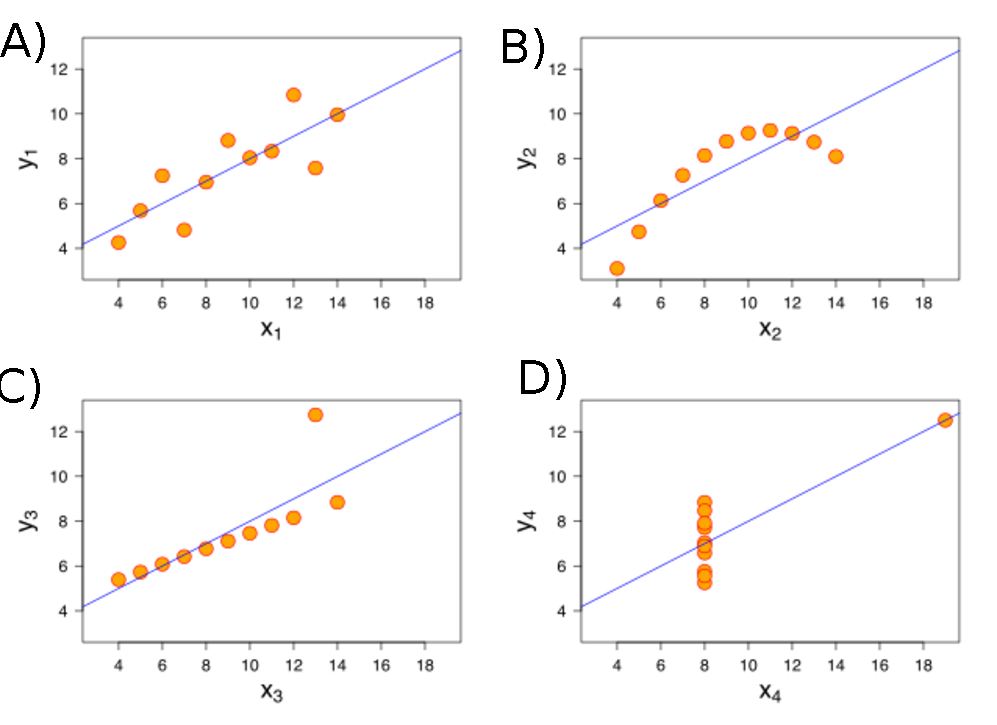
\includegraphics[scale=.65]{../slides/figures/anscombe_mod.pdf}
  \end{center}
   \end{figure}
   \\
Em todos os painéis, $\bar{x} = 9$, $\bar{y} = 7,5$, $s_x^2 = 110$ e $\operatorname{Cor}(X, Y) = 0,816$.
Isto é, todas as estatísticas sumárias relevantes atingem os mesmos valores.
Disto resulta que $\hat{\beta_0} = 3$ e $\hat{\beta_1}=0,5$ para todos os painéis.

\begin{enumerate}[label=\alph*)]
 \item (15 pontos) Comente sobre quais premissas básicas -- ou nenhuma -- da regressão linear aparentam estar sendo violadas em cada painel.
Justifique.
 \item (5 pontos) Os estimadores de máxima verossimilhança para os coeficientes no modelo
 \[ E[Y_i] = \beta_0 + \beta_1 X_i \]
 são 
 \begin{align*}
  \hat{\beta_0} &= \bar{y} - \hat{\beta_1}\bar{x},\\
  \hat{\beta_1} &= \frac{\sum_{i=1}^n (Y_i-\bar{y})(X_i-\bar{x})}{\sum_{i=1}^n \left(X_i - \bar{x}\right)^2}.
 \end{align*}
 Tais estimadores são viesados?
 Justifique.
 
 \textit{Dica:} Pode ser conveniente escrever
 $$\hat{\beta_1} = \frac{\sum_{i=1}^n \left(X_i-\bar{x}\right)Y_i}{s_x^2}.$$
 \end{enumerate}
\textcolor{red}{\textbf{Conceitos trabalhados}: Regressão linear; premissas da regressão linear; viés.}\\ \textcolor{purple}{\textbf{Nível de dificuldade}: médio.}\\
\textcolor{blue}{
\textbf{Resolução:}
Vamos responder a) por painel:
\begin{itemize}
 \item No painel A) não é possível identificar visualmente nenhuma violação clara das premissas do modelo de regressão;
 \item Já no painel B), podemos notar que a relação entre $Y$ e $X$ é não-linear, violando a premissa de linearidade, $E[Y] = \beta_0 + \beta_1X$;
 \item Em C) vemos um ponto aberrante, o que sugere violação da premissa de dados condicionalmente independentes e identicamente distribuídos (i.i.d);
 \item Finalmente em D) vemos que as premissas de linearidade e i.i.d. não parecem ser atendidas pois o ponto extremo à direita (chamado comumente de ``alavanca'') cria uma relação linear artificial entre $Y$ e $X$, que desapareceria se excluíssemos esse ponto.
\end{itemize}
Para responder b) temos dois caminhos: o mais simples é utilizar a dica dada no começo da prova e argumentar que como as distribuições de $\hat{\beta_0}$ e $\hat{\beta_1}$ são normais com média $\beta_0$ e $\beta_1$, os estimadores considerados são de fato não-viesados.
O segundo caminho, e mais complicado, é utilizar manipulações de esperanças, o que faremos a seguir.
Lembrando que $E[Y_i] = \beta_0 + \beta_1 X_i$, usando a dica dada na própria questão e passando o operador de esperança, temos
\begin{align*}
 E[\hat{\beta_1}] &= \frac{\sum_{i=1}^n \left(X_i-\bar{x}\right)E[Y_i]}{s_x^2},\\&= \frac{\sum_{i=1}^n \left(X_i-\bar{x}\right)\left(\beta_0 + \beta_1 X_i\right)}{s_x^2},\\
 &= \frac{\beta_0\sum_{i=1}^n\left(X_i-\bar{x}\right) + \beta_1\sum_{i=1}^nX_i\left(X_i-\bar{x}\right)}{\sum_{i=1}^n \left(X_i-\bar{x}\right)^2}.
\end{align*}
Como $\sum_{i=1}^n\left(X_i-\bar{x}\right) = 0$, temos que 
\begin{align*}
  E[\hat{\beta_1}] &= \frac{\beta_1\sum_{i=1}^nX_i\left(X_i-\bar{x}\right)}{\sum_{i=1}^n \left(X_i-\bar{x}\right)^2},\\
  &= \beta_1,
\end{align*}
porque\footnote{\textcolor{blue}{Prove isto, se quiser.}} $\sum_{i=1}^nX_i\left(X_i-\bar{x}\right) = \sum_{i=1}^n \left(X_i-\bar{x}\right)^2$.
Para $\hat{\beta_0}$, temos 
\begin{align*}
  E[\hat{\beta_0}] &= E[\bar{y}] - \beta_1\bar{x},\\
  &= \frac{\sum_{i=1}^n \beta_0 + \beta_1X_i}{n} - \beta_1\bar{x},\\
  &= \beta_0  + \frac{\sum_{i=1}^n \beta_1X_i}{n} - \beta_1\bar{x},\\
  &= \beta_0.
\end{align*}
\textbf{Nota:} A questão b) foi retirada~\textit{ipsis litteris} dos exercícios  2 e 3 da seção 11.2 de DeGroot (recomendados!). 
}

\section*{Questão Bônus: uma transformação útil.} 

Muitas vezes na aplicação de modelos de regressão é conveniente aplicar uma transformação à(s) variável(is) independente(s) de modo a facilitar a computação e/ou a interpretação das estimativas.

\begin{enumerate}[label=\alph*)]
 \item (10 pontos)  Considere uma regressão linear simples.
 Encontre  uma transformação $X^\prime = f(X)$ da variável independente de modo que $\hat{\beta_0^\prime}$ e $\hat{\beta_1^\prime}$ sejam independentes. 
 \item (5 pontos) Encontre o valor de $\hat{\beta_0^\prime}$ e $\hat{\beta_1^\prime}$ sob a transformação do item anterior.
 \item (5 pontos) Como essa transformação muda a interpretação dos coeficientes estimados? 
\end{enumerate}
\textcolor{red}{\textbf{Conceitos trabalhados}: Transformação de covariáveis; interpretação dos coeficientes.}\\
\textcolor{purple}{\textbf{Nível de dificuldade}: difícil.}\\
\textcolor{blue}{
\textbf{Resolução:}
Resposta de a): a partir da dica dada no começo da prova, sabemos que 
$$ \operatorname{Cov}\left(\hat{\beta_0^\prime}, \hat{\beta_1^\prime} \right)  = -\frac{\bar{x}^\prime\sigma^2}{s_x^2}.$$
Portanto, podemos considerar a transformação $X_i^\prime = X_i -\bar{x}$, de modo que $\bar{x}^\prime = 0$.
Chamamos este procedimento de ``centrar'' (em inglês, \textit{centering}) o preditor ou variável independente.
Disto, temos que $\operatorname{Cov}\left(\hat{\beta_0^\prime}, \hat{\beta_1^\prime} \right)  = 0$ e, portanto, $\hat{\beta_0^\prime}$ e $\hat{\beta_1^\prime}$ são não-correlacionadas.
Como a distribuição conjunta de $\hat{\beta_0^\prime}$ e $\hat{\beta_1^\prime}$ é bivariada normal (fato deduzido a partir dica), segue que  $\hat{\beta_0^\prime}$ e $\hat{\beta_1^\prime}$ são independentes.
Note que essa última conclusão se aplica somente a variáveis aleatórias normais, pois ~\textbf{neste caso}, correlação zero implica independência.\\
Para responder b) a respeito de $\hat{\beta_0^\prime}$ basta aplicar a fórmula dada para encontrar $\hat{\beta_0^\prime} = \bar{y}$.
Já para $\hat{\beta_1^\prime}$, precisamos notar que como $X_i^\prime = X_i - \bar{x}$,
\begin{align*}
 \hat{\beta_1^\prime} &= \frac{\sum_{i=1}^n (Y_i-\bar{y})(X_i^\prime-\bar{x}^\prime)}{\sum_{i=1}^n \left(X_i^\prime - \bar{x}^\prime\right)^2},\\
 &= \frac{\sum_{i=1}^n (Y_i-\bar{y})([X_i-\bar{x}]-0)}{\sum_{i=1}^n \left( [X_i-\bar{x}] - 0\right)^2},\\
 &= \hat{\beta_1},
\end{align*}
ou seja, a estimativa do coeficiente angular não muda!\\
Sobre c) vimos que $\hat{\beta_0}^\prime = \bar{y}$, isto é, o intercepto é a média da variável dependente.
Isso significa que $\beta_0$ pode ser entendido como a média da variável dependente quando a variável independente (a original!) atinge sua média.
Isso facilita bastante a interpretação, especialmente em situações em que $X$ nunca atinge zero em sua escala natural (por exemplo, quando $X$ é a altura de um indivíduo).
A interpretação de $\beta_1$ muda muito pouco, já que $X^\prime$ mantém as mesmas unidades que $X$.
Além disso, como vimos em b), $\hat{\beta_1^\prime} = \hat{\beta_1}$.
$\blacksquare$
}

\newpage
\section*{Fórmulas úteis}
\textbf{Como usar este catálogo:} as fórmulas dadas aqui estão propositalmente privadas do seu contexto.
O objetivo desta coleção é ajudar você a lembrar das expressões.
Entretanto, saber quais expressões são utilizadas em que contexto é sua tarefa.
\begin{itemize}
 \item $ \bar{X}_n = \frac{1}{n} \sum_{i=1}^n X_i$;
 \item $\hat{\sigma}^\prime = \sqrt{\frac{1}{n-1}\sum_{i=1}^n \left(X_i - \bar{X}_n\right)^2}$;
 \item $S_X^2 = \sum_{i=1}^m (X_i-\bar{X}_m)^2$;
 \item $S_Y^2 = \sum_{j=1}^n (Y_j-\bar{Y}_n)^2$;
 \item $U = \frac{\sqrt{m + n - 2}(\bar{X}_m - \bar{Y}_n)}{\sqrt{\left(\frac{1}{m} + \frac{1}{n}\right) (S_X^2 + S_Y^2)}}$;
 \item $ V = \frac{S_X^2/(m-1)}{S_Y^2/(n-1)}$;
 \item $\bar{x} = (1/n)\sum_{i=1}^n X_i$;
 \item $\bar{y} = (1/n)\sum_{i=1}^n Y_i$.
\end{itemize}


% \bibliographystyle{apalike}
% \bibliography{refs}

\end{document}          
